\documentclass[a4paper]{article}
\usepackage{graphicx}
\begin{document}
\section{Turing Machines: The Simplest Computers}
\label{sec:simplest}
Turing machines are the simplest and most widely used theoretical models of computing. Far too slow and unwieldy ever to be embodied in a real device, these conceptual machines nevertheless seem to capture everything we mean by the term \textit{computation}. Not only do Turing machines occupy the top level of the Chomsky hierarchy, but they also seem capable of computing any function which is computable by any other conceptual scheme.

\begin{figure}
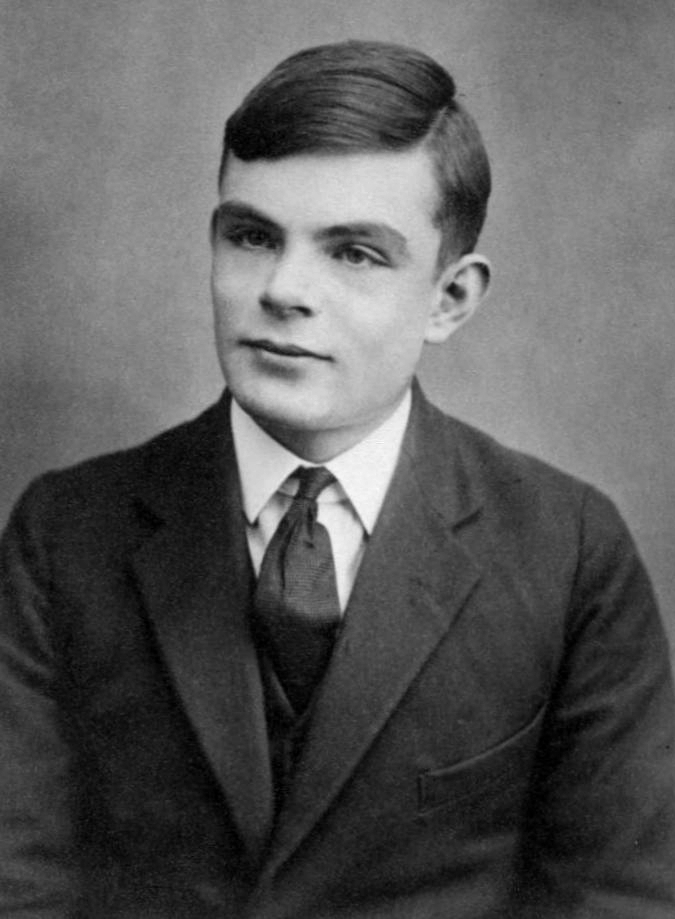
\includegraphics[width=10cm]{Alan_Turing_Aged_16.jpg}
\caption{Turing machines are named after Alan Turing}
\label{figure:turing}
\end{figure}



\section{Alan Turing}
The Turing machines described in section \ref{sec:simplest} are named after Alan Turing.
\end{document}